\section{Critic conditioning across players}
\label{sec:observer}
\subsection{Critic information and decision times}
Baisero and Amato analyze the bias from substituting state critics for history
critics and develop a history-state formulation \cite{baisero2022asymmetric}.
Lyu et al. show that state-based multi-agent critics can bias policy gradients
and, even when unbiased, can increase their variance \cite{lyu2022critics}.
Our example studies a specific instance of this conditioning problem: a
player-relative return crosses between two players' observations. It makes the
failure explicit with exact conditional values and a policy update that reduces
true expected payoff. Its return recurrence is checked in all three simulator
backends.

Sutton, Precup and Singh formalize temporally extended decisions with options
and semi-Markov models \cite{sutton1999options}. Learner-decision returns use a
related temporal organization: opponent moves lie inside an interval between
the learner's actions. Our analysis focuses on the information used at those
boundaries, with exactness established for the finite example and Koi-Koi
assessed in the fixed-opponent comparison.

\subsection{Exact update reversal}
Correct payoff signs do not ensure that the next acting player's observation
contains the information needed by the current learner's target. The following
finite game isolates this issue without critic fitting or sampled trajectories.

A learner privately observes a uniform bit $X$ and takes a public binary action
$A$, with $\pi(A=1\mid X=x)=\sigma(c_x\theta)$, where $c_0=1$ and
$c_1=-1/100$. Both signal-dependent policies share the scalar parameter $\theta$.
The opponent sees $A$, takes one forced action, and the game ends with learner
payoff $R\in\{-1,+1\}$.
Define $\Pr(R=+1\mid X=x,A=a)=(1+\mu_{xa})/2$, where
\begin{equation}
 (\mu_{xa})=\begin{pmatrix}0.20&0.21\\1&-1\end{pmatrix}.
\end{equation}
At $\theta=0$, the exact learner values are
$v_0=0.205,v_1=0$. The opponent's exact own-payoff value is $-m_A$, with
$m_0=0.60,m_1=-0.395$. Signed GAE at the learner action therefore gives
\begin{equation}
 \widehat A=\lambda R+(1-\lambda)m_A-v_X.
 \label{eq:observer-advantage}
\end{equation}
For the objective $J=\mathbb E[R]$ and $\lambda=0.95$, direct differentiation
and exact enumeration give
\begin{align}
 J'(0)&=\frac{3}{800}=0.00375,\\
 \mathbb E[\widehat A\,\partial_\theta\log\pi(A\mid X)]
 &=-\frac{8301}{3200000}=-0.0025940625.
\end{align}
The expected update has the opposite sign to the true gradient
(Figure~\ref{fig:observer-reversal}). A sufficiently small positive step
in that direction therefore reduces true expected payoff. The opponent critic
averages over $X$, changing the relative targets for the two actions when the
learner knows $X=0$. This result concerns the population score-function update
before PPO clipping and empirical advantage normalization.

\begin{figure}[htbp]
\centering
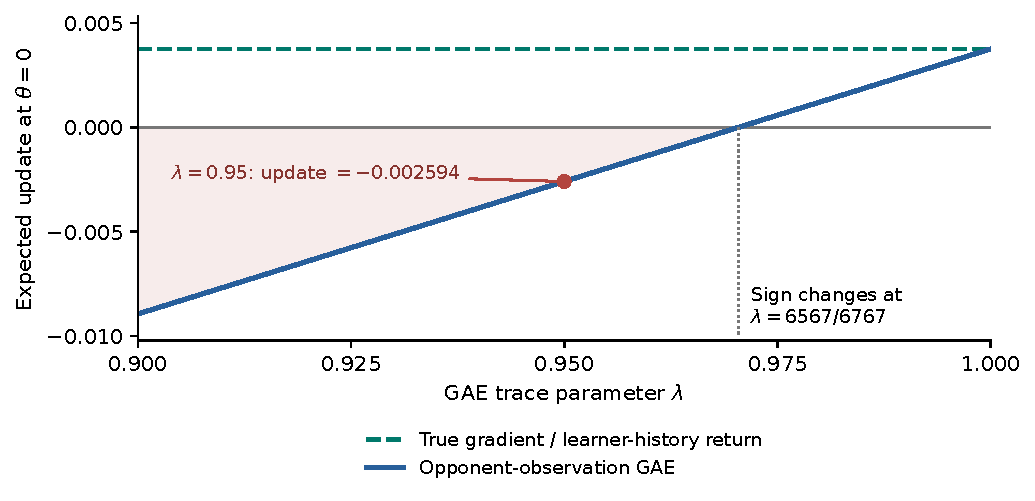
\includegraphics[width=0.88\linewidth]{generated/observer_reversal.pdf}
\caption{Exact expectations in the two-step game. The true gradient is positive,
but opponent-observation GAE points in the opposite direction for
$\lambda<6567/6767\approx0.9704$. Both critics are exact for their respective
observations. The marked $\lambda=0.95$ case therefore reduces expected payoff
under a sufficiently small positive update.}
\label{fig:observer-reversal}
\end{figure}

Three controls recover the true expectation for the complete game: $\lambda=1$, a
single learner-to-terminal transition, and an intermediate critic conditioned
on both $X$ and $A$. The Python, native CPU and CUDA implementations reproduce
the return calculation. The scalar expectation also agrees with direct objective
differentiation. Appendix~\ref{app:observer} gives the derivation and a
learner-decision implementation with explicit tail masks.
The Koi-Koi match results above use the original signed estimator.
Appendix~\ref{sec:learner} compares the return constructions under fixed-opponent
training.

The $\lambda=1$ cancellation requires reaching termination. Cutting this same
game after the learner action leaves the opponent-observation bootstrap and
a negative expected update, even at $\lambda=1$. Retaining the learner history
restores the correct gradient. Appendix~\ref{app:trace} separates the internal
bootstrap terms from this rollout-boundary term.

\subsection{Directional measurements in the retained agents}
\label{sec:directional}
To connect the finite example to actual play, we collect 4,096 complete sampled
self-play matches from each retained agent, sharing initial deals across the
two agents. For a fixed public feature $f$, the local policy
$\pi_\theta(a\mid o)\propto\pi_0(a\mid o)\exp(\theta f(o,a))$ has score
$f(o,a)-\mathbb E_{\pi_0}f(o,A)$. The five features are a continuation indicator
and one base-probability preference feature for each decision phase. Features
and critics stay fixed. We sum score times advantage separately for each seat,
then average the two unilateral responses against the frozen other seat.

Complete terminal Monte Carlo contributions are compared with full-match
GAE0.95 and 128-step-window GAE0.95/GAE1, using independently assigned cutoff
positions. One 70-coordinate simultaneous bootstrap family covers all means
and differences across both agents. Every Monte Carlo mean and every paired
difference interval includes zero. Thus these probes do not establish the
finite example's reversal in the retained agents. The measurement concerns
these local policy directions before PPO clipping and normalization; it does
not identify observer mismatch separately from critic approximation error.
All 8,192 matches are replayed on native CPU, and independent scalar score and
return calculations agree to $8.9\times10^{-16}$. Full coordinates and the
fixed design are in \path{docs/DIRECTIONAL_RETURN_RESULTS.rst}.

\subsection{Do return repairs improve learned play?}
The exact counterexample motivates two implementations: returns between
learner decisions, and a critic that maintains each player's viewpoint through
all primitive decisions. Both are tested from the two retained parents against
unchanged parents and signed-return controls. Each new arm receives
8.52 million simulator decisions. Separate paired evaluations contain 160,000
full matches per study. The fixed-observer contrast holds critic fitting fixed;
the learner-decision procedure also changes critic fitting and optimization.

Learner-decision returns have positive mean win changes in all eight primary
comparisons, but only one lower 95\% bound is positive. Against Point, gains
over the two parents are 0.920 percentage points [0.125, 1.755] and 0.325
[$-0.480$, 1.165]. All four learner-minus-response win intervals include zero.
The fixed-observer comparison has no positive lower bound among its eight
primary intervals. These results separate the exact analytical repair from
an additional playing-strength gain. Appendices~\ref{sec:training}
and~\ref{sec:observer-selfplay} retain the complete training protocols,
matched controls, point outcomes and comparison tables.
